\section{Plattform Hadoop"=Benchmark}
\label{sec:hadoopBenchmark}

\citeauthor{Zhang2016} haben im Rahmen ihrer gesamten Forschungsarbeit an der Selfbalancing"=Komponente darüber hinaus auch die Open"=Source"=Plattform Hadoop"=Benchmark\footnote{\url{https://github.com/Spirals-Team/hadoop-benchmark}} entwickelt.
Sie dient zur einfachen und schnellen Ausführung eines Hadoop"=Clusters und wurde speziell zum Einsatz in der Forschung erstellt.
Dadurch kann sie auch mit geringem Aufwand an eigene Bedürfnisse angepasst werden.

Zur Ausführung des Clusters wird die Virtualisierungs"=Software Docker und das dazugehörige Tool \emph{Docker Machine} genutzt.
Durch die Virtualisierung wird für jeden Hadoop"=Node eine Docker"=Machine gestartet, auf der der Hadoop"=Node wiederum in einem Docker"=Container ausgeführt wird.
Verbunden werden die Nodes dabei mithilfe eines \emph{Docker  Swarm}s\footnote{\url{https://docs.docker.com/engine/swarm/}}.

\begin{figure}[h]
    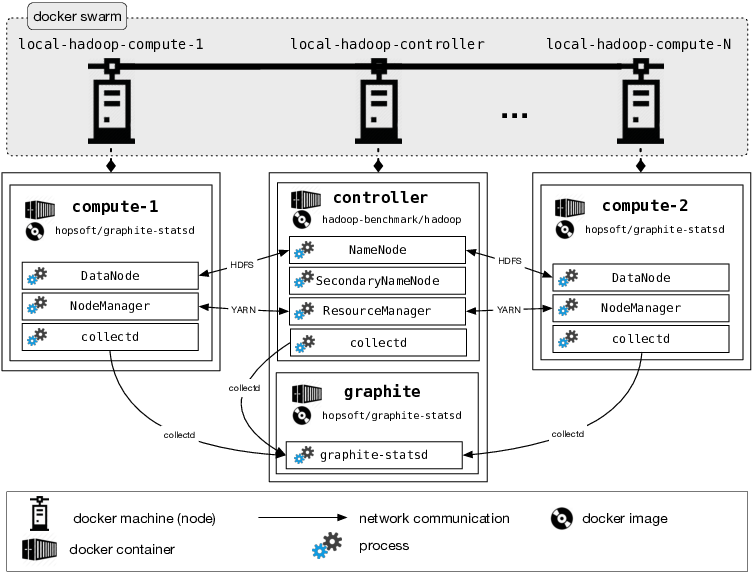
\includegraphics{./resources/hadoopBenchmarkArch.png}
    \caption[High"=Level"=Architektur von Hadoop"=Benchmark]
    {High"=Level"=Architektur von Hadoop"=Benchmark (entnommen aus \cite{abb:hadoopBenchmarkArch})}
    \label{fig:hadoopBenchmarkArchitecture}
\end{figure}

Docker"=Machine nutzt hierbei VirtualBox\footnote{\url{https://www.virtualbox.org/}}, um virtuelle Maschinen zu starten, die mit dem Betriebssystem \emph{Boot2Docker} ausgestattet sind.
Boot2Docker selbst ist eine einfache Linux"=Distribution, die zum Ausführen von Docker"=Containern auf dem System \cite{DockerMachineGettingStartedVm}.

Mit \emph{Graphite}\footnote{\url{https://graphiteapp.org/}} ist zudem ein Monitoring"=Tool enthalten, mit dem die Systemwerte wie CPU- oder Speicher"=Auslastung des Clusters überwacht und analysiert werden kann.
Jeder Hadoop"=Container enthält dazu das Tool \emph{collectd}\footnote{\url{https://collectd.org/}}, was das Monitoring des Containers auf Systemebene übernimmt und die Daten an Graphite übermittelt.

Da mithilfe der Plattform auch unterschiedliche Hadoop"=Konfigurationen ausgeführt werden können, ist die Plattform in mehrere Szenarien unterteilt.
Jedes Szenario stellt eine vollständig anpassbare Hadoop"=Konfiguration dar.
Ein Szenario enthält dafür eine \emph{Dockerfile}, aus der die Docker"=Images und -Container erstellt werden, weitere für Hadoop benötigte Daten und Einstellungen, sowie dazugehörige generelle Einstellungen des Szenarios.
Die Plattform enthält bereits mehrere Szenarien, \uA Hadoop in der Version 2.7.1 ohne Anpassungen sowie ein darauf basierendes Szenario mit der Selfbalancing"=Komponente.
Aufgrund eines der Kernkonzepte von Docker, wonach Docker"=Images auf einem passenden, bereits vorhandenen Images aufbauen können bzw. sollten \cite{DockerdevBestPractice}, ist es möglich, neue Szenarien basierend auf bereits vorhandenen zu entwickeln.

Zum Starten des Clusters ist zudem ein Script enthalten, welches basierend auf dem zu nutzenden Szenario das Cluster in der entsprechenden Konfiguration startet.

In der Plattform Hadoop"=Benchmark sind auch bereit folgende Benchmarks integriert:

\begin{itemize}
    \item Hadoop"=Mapreduce"=Examples
    \item Intel HiBench\footnote{\url{https://github.com/intel-hadoop/HiBench}}
    \item \gls{SWIM} \footnote{\url{https://github.com/SWIMProjectUCB/SWIM}}
\end{itemize}

Die Benchmarks werden ebenfalls mithilfe der in der Plattform enthaltenen Scripte gestartet.
Hierbei besitzt jeder Benchmark ein eigenes Start"=Script, das den Benchmark in einem Docker"=Container startet und die entsprechende Anwendung so dem Cluster zur Ausführung übergibt.
Die Ausführung einer Anwendung mithilfe des entsprechenden Start"=Scriptes sowie das Beenden einer Anwendung ist in \cref{app:hadoopCmds} beispielhaft aufgezeigt.

Genauere Informationen zu den in der Plattform enthaltenen Benchmarks sind in \cref{sec:appOverview} erläutert.
